\chapter{रासायनिक निकाय का वर्णन: प्रगति, सक्रियताएँ, Q और K}\label{ch:b1:extent-q-and-k}

हाइड्रोजन संयंत्र में प्राकृतिक गैस और भाप को लाल-तप्त नलियों में भेजा जाता है;
बाहर जो निकलता है वह कभी शुद्ध हाइड्रोजन नहीं, बल्कि हाइड्रोजन, कार्बन
मोनॉक्साइड, कार्बन डाइऑक्साइड, बिना अभिक्रिया वाली मेथेन और भाप का मिश्रण होता है,
जिसके अनुपात इंजीनियरों को अगली इकाई का अभिकल्पन करने से पहले जानने होते हैं।
रिएक्टर से निकलने वाले संघटन --- रासायनिक निकाय की अंतिम अवस्था --- का
पूर्वानुमान ही इस अध्याय का विषय है। इसके लिए निकाय का सटीक
वर्णन (उसके चर और उसका संघटन), एक ऐसी अकेली
संख्या जो मापे कि अभिक्रिया कितनी आगे बढ़ी (प्रगति), और वह
नियम जो बताए कि अभिक्रिया कहाँ रुकती है (साम्य स्थिरांक), आवश्यक हैं।
ये साधन विलयनों के आगे के हर अध्याय में प्रयुक्त होते हैं।

\begin{recall}
पुस्तक 1 (कक्षा 10) ने प्रगति सारणी से अभिक्रिया का अनुसरण किया था और
\omterm{def:b1:extent-q-and-k:max-extent}{सीमांत अभिकारक} खोजा था; पुस्तक 1 (कक्षा 12) ने अपूर्ण अभिक्रिया के \omterm{def:b1:extent-q-and-k:quotient}{अभिक्रिया भागफल}
$Q$ और साम्य स्थिरांक $K$ का परिचय दिया था। भौतिकी से
हम आदर्श गैस नियम $pV = nRT$ लेते हैं, जहाँ $R =
\qty{8.314}{J/(mol.K)}$।
\end{recall}

\begin{omfigure}
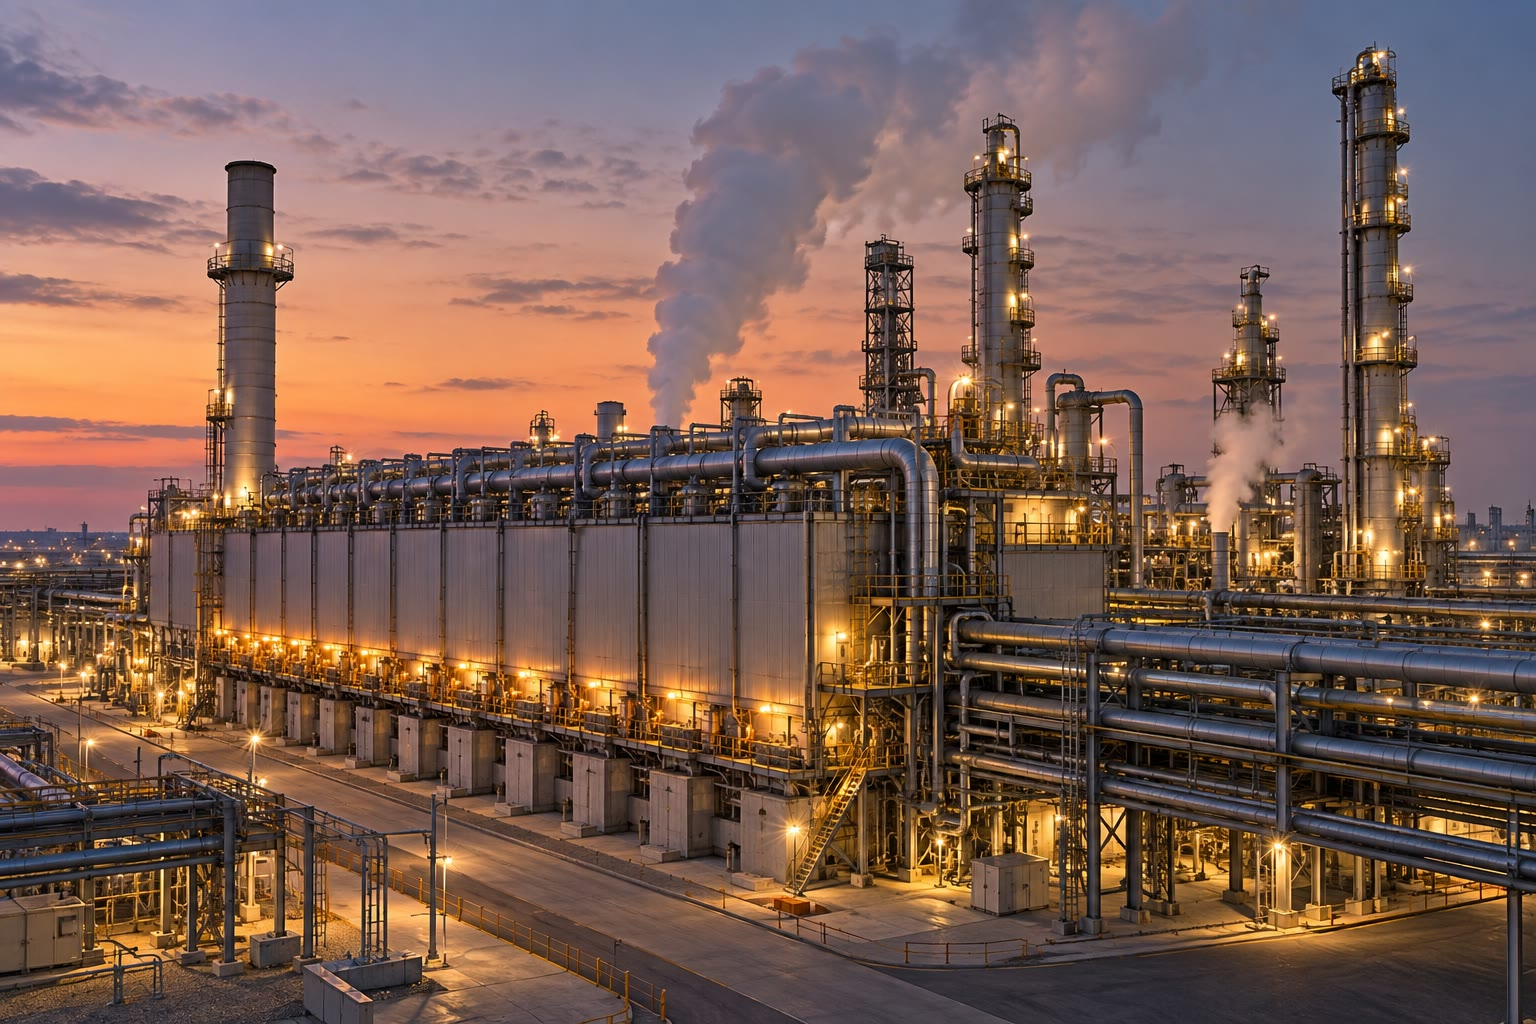
\includegraphics[width=0.6\linewidth]{images/book2/ai/b1-07-hydrogen-plant.jpg}

{\small संध्या के समय एक हाइड्रोजन संयंत्र। प्राकृतिक गैस और भाप लंबी
रिफ़ॉर्मर भट्ठी में अभिक्रिया करती हैं; दूसरा रिएक्टर कार्बन मोनॉक्साइड को बदलता है;
निकास का संघटन ठीक उसी प्रकार की अंतिम अवस्था है जिसका परिकलन इस
अध्याय में किया जाता है।}
\end{omfigure}

\section{निकाय का वर्णन}

\begin{definition}[निकाय, प्रावस्था]\label{def:b1:extent-q-and-k:system}
\emph{भौतिक-रासायनिक निकाय}\index{भौतिक-रासायनिक निकाय} आकाश के किसी
चुने हुए क्षेत्र में स्थित द्रव्य है, शेष उसका परिवेश है। यदि वह परिवेश के साथ
द्रव्य का कोई विनिमय नहीं करता (ऊर्जा का कर सकता है), तो वह \emph{बंद निकाय}\index{बंद निकाय}
है। \emph{प्रावस्था}\index{प्रावस्था} निकाय का वह भाग है जिसमें \omterm{def:b1:extent-q-and-k:variables}{गहन
चर} सतत रूप से बदलते हैं: गैसों का मिश्रण एक प्रावस्था है, दो अमिश्रणीय
द्रव दो प्रावस्थाएँ हैं, हर ठोस अपनी अलग प्रावस्था है।
\end{definition}

\begin{definition}[गहन और विस्तीर्ण चर]\label{def:b1:extent-q-and-k:variables}
कोई अवस्था-चर \emph{विस्तीर्ण}\index{विस्तीर्ण चर} है यदि वह
निकाय के आकार के समानुपाती है (द्रव्यमान, आयतन, पदार्थ की
मात्रा) और \emph{गहन}\index{गहन चर} है यदि नहीं
(ताप, दाब, सांद्रता, घनत्व, \omterm{def:b1:extent-q-and-k:composition}{मोल अंश})। दो विस्तीर्ण चरों का
अनुपात गहन होता है।
\end{definition}

\begin{definition}[संघटन के चर]\label{def:b1:extent-q-and-k:composition}
किसी \omterm{def:b1:extent-q-and-k:system}{प्रावस्था} के किसी घटक $i$ के लिए, जिस \omterm{def:b1:extent-q-and-k:system}{प्रावस्था} में उसके सभी
घटकों की मात्राएँ $n_j$ हैं:
\begin{itemize}
  \item उसका \emph{मोल अंश}\index{मोल अंश} $x_i = n_i/\sum_j
        n_j$ है, और उसका \emph{द्रव्यमान अंश}\index{द्रव्यमान अंश} $w_i =
        m_i/\sum_j m_j$; दोनों 0 और 1 के बीच होते हैं और उनका योग 1 होता है;
  \item आयतन $V$ वाले विलयन में उसकी \emph{मोलर
        सांद्रता}\index{मोलर सांद्रता} $c_i = [i] = n_i/V$ है,
        \unit{mol/L} में;
  \item कुल दाब $p$ पर गैस मिश्रण में उसका \emph{आंशिक
        दाब}\index{आंशिक दाब} $p_i = x_i\,p$ है।
\end{itemize}
\end{definition}

\begin{proposition}[आदर्श गैसों के आंशिक दाब]\label{prop:b1:extent-q-and-k:dalton}
आयतन $V$ और ताप $T$ पर आदर्श गैसों के मिश्रण में किसी
घटक का \omterm{def:b1:extent-q-and-k:composition}{आंशिक दाब} वह दाब है जो वह पूरे आयतन में अकेले
डालता, $p_i = n_iRT/V$, और \omterm{def:b1:extent-q-and-k:composition}{आंशिक दाबों} का योग
कुल दाब होता है: $\sum_i p_i = p$।
\end{proposition}

\begin{proof}
मिश्रण के लिए $pV = (\sum_j n_j)RT$, इसलिए $p_i = x_i p = \frac{n_i}{\sum_j
n_j}\cdot\frac{(\sum_j n_j)RT}{V} = \frac{n_iRT}{V}$, और $\sum_i x_i = 1$
से $\sum_i p_i = p$ मिलता है।
\end{proof}

\begin{example}[वायु]\label{ex:b1:extent-q-and-k:air}
शुष्क वायु में आयतन के अनुसार (अर्थात् आदर्श गैसों के लिए मात्रा के अनुसार)
78.08\,\% डाइनाइट्रोजन, 20.95\,\% डाइऑक्सीजन और 0.93\,\% आर्गन होती है।
\qty{1.013}{bar} पर डाइऑक्सीजन का \omterm{def:b1:extent-q-and-k:composition}{आंशिक दाब} $0.2095 \times
1.013 = \qty{0.212}{bar}$ है; किसी पहाड़ पर जहाँ दाब
\qty{0.70}{bar} है, वह \qty{0.147}{bar} रह जाता है, यद्यपि संघटन
वही है।
% ledger: air:N2, air:O2, air:Ar, const:atm
\end{example}

\section{अभिक्रिया की प्रगति}

\begin{definition}[रससमीकरणमितीय संख्याएँ, प्रगति]\label{def:b1:extent-q-and-k:extent}
अभिक्रिया को $0 = \sum_i \nu_i\,\mathrm{A}_i$ लिखा जाता है, जहाँ
\emph{रससमीकरणमितीय संख्या}\index{रससमीकरणमितीय संख्या} $\nu_i$ (स्पीशीज़
$\mathrm{A}_i$ की) अभिकारक के लिए ऋणात्मक और उत्पाद के लिए धनात्मक होती है:
\ce{N2 + 3H2 -> 2NH3} में $\nu(\ce{N2}) = -1$, $\nu(\ce{H2}) = -3$,
$\nu(\ce{NH3}) = +2$। किसी \omterm{def:b1:extent-q-and-k:system}{बंद निकाय} में, जहाँ केवल यही अभिक्रिया
होती है, मात्राएँ इस प्रकार बदलती हैं:
\[
  n_i = n_{i,0} + \nu_i\,\xi ,
\]
जो \emph{अभिक्रिया की प्रगति}\index{अभिक्रिया की प्रगति}
$\xi$ (मोल में) को परिभाषित करता है, जो आरंभ में शून्य है और हर स्पीशीज़ के लिए समान है।
\end{definition}

\begin{definition}[अधिकतम प्रगति, सीमांत अभिकारक]\label{def:b1:extent-q-and-k:max-extent}
\emph{अधिकतम प्रगति}\index{अधिकतम प्रगति} $\xi_{\max}$, $\xi$ का वह सबसे बड़ा
मान है जिस पर कोई मात्रा ऋणात्मक नहीं होती: $\xi_{\max} = \min_{\nu_i <
0} n_{i,0}/|\nu_i|$। जो अभिकारक $\xi_{\max}$ पर शून्य तक पहुँचता है, वह
\emph{सीमांत अभिकारक}\index{सीमांत अभिकारक} है। जब प्रगति
ऋणात्मक भी हो सकती है (प्रतीप अभिक्रिया), तब $\xi_{\min} = -\min_{\nu_i > 0}
n_{i,0}/\nu_i$।
\end{definition}

\begin{method}[प्रगति सारणी]\label{met:b1:extent-q-and-k:progress-table}
किसी \omterm{def:b1:extent-q-and-k:system}{बंद निकाय} में अभिक्रिया का अनुसरण करने के लिए:
\begin{enumerate}
  \item संतुलित समीकरण लिखिए, और उसके नीचे हर स्पीशीज़ के लिए एक स्तंभ;
  \item पहली पंक्ति: प्रारंभिक मात्राएँ $n_{i,0}$;
  \item दूसरी पंक्ति: प्रगति $\xi$ पर मात्राएँ, $n_{i,0} + \nu_i\xi$;
  \item गैसों के लिए कुल मात्रा $n_{\text{कुल}}(\xi)$ का एक स्तंभ जोड़िए;
  \item $\xi_{\max}$ (और $\xi_{\min}$) परिकलित कीजिए और \omterm{def:b1:extent-q-and-k:max-extent}{सीमांत
        अभिकारक} पहचानिए;
  \item अंतिम पंक्ति: अंतिम प्रगति $\xi_f$ पर अंतिम मात्राएँ (जो प्रगति
        साम्य की शर्त से मिलती है, या अभिक्रिया पूर्ण हो तो
        $\xi_{\max}$ के बराबर होती है)।
\end{enumerate}
\end{method}

\begin{example}[अमोनिया का संश्लेषण]\label{ex:b1:extent-q-and-k:ammonia}
\ce{N2} के \qty{2.0}{mol} और \ce{H2} के \qty{3.0}{mol} से:
\begin{center}
\begin{tabular}{lcccc}
\hline
 & \ce{N2} & \ce{3H2} & \ce{2NH3} & कुल \\
\hline
प्रारंभिक & 2.0 & 3.0 & 0 & 5.0 \\
प्रगति $\xi$ & $2.0 - \xi$ & $3.0 - 3\xi$ & $2\xi$ & $5.0 - 2\xi$ \\
\hline
\end{tabular}
\end{center}
$\xi_{\max} = \min(2.0/1,\ 3.0/3) = \qty{1.0}{mol}$: डाइहाइड्रोजन सीमांत है।
यदि अभिक्रिया पूर्ण होती, तो अंतिम अवस्था में \qty{1.0}{mol}
\ce{N2} और \qty{2.0}{mol} \ce{NH3} होते।
\end{example}

\begin{definition}[अंतिम प्रगति अनुपात, लब्धि]\label{def:b1:extent-q-and-k:fractional-extent}
किसी अभिक्रिया का \emph{अंतिम प्रगति अनुपात}\index{अंतिम प्रगति अनुपात}
$\tau = \xi_f/\xi_{\max}$ है, जो 0 और 1 के बीच होता है। किसी संश्लेषण में किसी उत्पाद की
\emph{लब्धि}\index{लब्धि} प्राप्त मात्रा और उस मात्रा का अनुपात है
जो \omterm{def:b1:extent-q-and-k:max-extent}{सीमांत अभिकारक} अभिक्रिया के पूर्ण होने पर देता;
यदि पृथक्करण के दौरान उत्पाद की कोई हानि न हो, तो यह $\tau$ के बराबर होती है।
\end{definition}

\section{सक्रियताएँ}

\begin{definition}[मानक अवस्था, सक्रियता]\label{def:b1:extent-q-and-k:activity}
किसी स्पीशीज़ की \emph{सक्रियता}\index{सक्रियता} $a_i$ एक विमाहीन
संख्या है जो साम्य नियमों की अभिव्यक्ति में यह मापती है कि वह स्पीशीज़ कितनी
उपलब्ध है; इसे एक \emph{मानक
अवस्था}\index{मानक अवस्था} के सापेक्ष परिभाषित किया जाता है, जो विचाराधीन ताप पर और
मानक दाब $p^\circ = \qty{1}{bar}$ पर एक संदर्भ अवस्था है। इस
पुस्तक में प्रयुक्त आदर्श सन्निकटनों में:
\begin{itemize}
  \item गैस के लिए $a_i = p_i/p^\circ$ (मानक अवस्था $p^\circ$ पर शुद्ध
        आदर्श गैस है);
  \item तनु विलयन में विलेय के लिए $a_i = c_i/c^\circ$, जहाँ
        $c^\circ = \qty{1}{mol/L}$;
  \item तनु विलयन के विलायक के लिए, और अपनी \omterm{def:b1:extent-q-and-k:system}{प्रावस्था} में अकेले शुद्ध ठोस या
        शुद्ध द्रव के लिए, $a_i = 1$।
\end{itemize}
\end{definition}
% ledger: const:pstd

\begin{remark}[आदर्श और वास्तविक]\label{rem:b1:extent-q-and-k:ideal}
ये व्यंजक आदर्श गैसों और तनु विलयनों के लिए मान्य हैं।
सांद्र विलयनों में आयन एक-दूसरे को आकर्षित और प्रतिकर्षित करते हैं और
\omterm{def:b1:extent-q-and-k:activity}{सक्रियता} $c_i/c^\circ$ से हट जाती है; \omterm{def:b1:extent-q-and-k:activity}{सक्रियता} गुणांकों से लिखे जाने वाले संशोधनों
का अध्ययन द्वितीय वर्ष के खंड में रासायनिक
विभव के साथ होता है। इस पुस्तक में प्रयुक्त सांद्रताओं (लगभग
\qty{0.1}{mol/L} से कम) के लिए आदर्श व्यंजक कुछ प्रतिशत तक सही हैं।
\end{remark}

\section{अभिक्रिया भागफल और साम्य स्थिरांक}

\begin{definition}[अभिक्रिया भागफल]\label{def:b1:extent-q-and-k:quotient}
निकाय की किसी दी गई अवस्था में अभिक्रिया
$0 = \sum_i \nu_i\,\mathrm{A}_i$ का \emph{अभिक्रिया भागफल}\index{अभिक्रिया भागफल} है
\[
  Q = \prod_i a_i^{\nu_i} ,
\]
अर्थात् उत्पादों की \omterm{def:b1:extent-q-and-k:activity}{सक्रियताओं} का गुणनफल भाग अभिकारकों की \omterm{def:b1:extent-q-and-k:activity}{सक्रियताओं} का गुणनफल, हर एक
अपने रससमीकरणमितीय गुणांक की घात पर।
\end{definition}

\begin{example}[तीन भागफल]\label{ex:b1:extent-q-and-k:quotients}
\ce{N2(g) + 3H2(g) <=> 2NH3(g)} के लिए: $Q = \dfrac{(p_{\ce{NH3}}/p^\circ)^2}
{(p_{\ce{N2}}/p^\circ)(p_{\ce{H2}}/p^\circ)^3}$।
\ce{CH3COOH(aq) + H2O(l) <=> CH3COO^-(aq) + H3O+(aq)} के लिए: $Q =
\dfrac{[\ce{CH3COO-}][\ce{H3O+}]}{[\ce{CH3COOH}]\,c^\circ}$, क्योंकि विलायक
की \omterm{def:b1:extent-q-and-k:activity}{सक्रियता} 1 है। \ce{CaCO3(s) <=> CaO(s) + CO2(g)} के लिए: $Q =
p_{\ce{CO2}}/p^\circ$, क्योंकि ठोसों की \omterm{def:b1:extent-q-and-k:activity}{सक्रियता} 1 है।
\end{example}

\begin{definition}[मानक साम्य स्थिरांक]\label{def:b1:extent-q-and-k:equilibrium-constant}
किसी अभिक्रिया का \emph{मानक साम्य स्थिरांक}\index{मानक साम्य स्थिरांक}
$K^\circ$ वह मान है जो निकाय के साम्य में होने पर उसका \omterm{def:b1:extent-q-and-k:quotient}{अभिक्रिया
भागफल} लेता है। यह विमाहीन है और
केवल अभिक्रिया और ताप पर निर्भर करता है।
\end{definition}

\begin{theorem}[द्रव्य-अनुपाती क्रिया का नियम]\label{thm:b1:extent-q-and-k:mass-action}
किसी दिए गए ताप पर, जिस निकाय में कोई अभिक्रिया दोनों दिशाओं में
हो सकती है, वह तब तक विकसित होता है जब तक $Q = K^\circ(T)$ न हो जाए; साम्य पर,
प्रारंभिक संघटन चाहे जो हो,
\[
  \prod_i a_{i,\text{साम्य}}^{\nu_i} = K^\circ(T) .
\]
\end{theorem}
\admitted

\begin{proposition}[विकास की दिशा]\label{prop:b1:extent-q-and-k:direction}
जिस निकाय में $Q < K^\circ$ हो, वह अग्र दिशा में विकसित होता है ($\xi$
बढ़ता है); यदि $Q > K^\circ$, तो वह प्रतीप दिशा में विकसित होता है; यदि
$Q = K^\circ$, तो वह साम्य में है।
\end{proposition}
\admitted

\begin{remark}[ये नियम कहाँ से आते हैं]\label{rem:b1:extent-q-and-k:origin}
दोनों कथन ऊष्मागतिकी के दूसरे नियम से, अभिक्रिया की मुक्त ऊर्जा और स्पीशीज़ के
रासायनिक विभवों के माध्यम से, निकलते हैं: इनकी
व्युत्पत्ति द्वितीय वर्ष के खंड में है, जो ऊष्मागतिक आँकड़ों की सारणियों से
$K^\circ$ भी देता है और समझाता है कि ताप के साथ यह कैसे बदलता है। यहाँ
इन्हें नियमों के रूप में प्रयुक्त किया गया है।
\end{remark}

\begin{omfigure}
\begin{tikzpicture}[font=\small, >={Stealth}]
  \draw[->, thick] (0,0) -- (11,0) node[right] {$Q$};
  \draw[thick, omThm] (5.5,0.25) -- (5.5,-0.25) node[below] {$K^\circ$};
  \draw[->, omDef, thick] (1.0,0.55) -- (4.6,0.55);
  \node[above, omDef] at (2.8,0.6) {$Q < K^\circ$: अग्र};
  \draw[->, omProp, thick] (10.0,0.55) -- (6.4,0.55);
  \node[above, omProp] at (8.2,0.6) {$Q > K^\circ$: प्रतीप};
  \node[below] at (0,-0.1) {0};
\end{tikzpicture}

{\small भागफल स्थिरांक की ओर बढ़ता है: $Q <
K^\circ$ वाला निकाय उत्पाद बनाता है, $Q > K^\circ$ वाला उन्हें खपाता है।}
\end{omfigure}

\begin{proposition}[स्थिरांकों का संयोजन]\label{prop:b1:extent-q-and-k:combine-k}
यदि $K_1^\circ$ और $K_2^\circ$ अभिक्रियाओं (1) और (2) के स्थिरांक हैं, तो:
(1) की प्रतीप अभिक्रिया का स्थिरांक $1/K_1^\circ$ है; अभिक्रिया $n \times
(1)$ का $(K_1^\circ)^n$; योग $(1) + (2)$ का $K_1^\circ K_2^\circ$।
\end{proposition}

\begin{proof}
प्रतीप अभिक्रिया का भागफल $\prod a_i^{-\nu_i} = 1/Q_1$ है;
$n \times (1)$ का $\prod a_i^{n\nu_i} = Q_1^n$; योग का
$\prod a_i^{\nu_{i,1} + \nu_{i,2}} = Q_1 Q_2$। इन सर्वसमिकाओं को
साम्य पर लिखने से, जहाँ हर भागफल अपने स्थिरांक के बराबर है, परिणाम मिलता है।
\end{proof}

\begin{proposition}[एक ही साम्य अवस्था]\label{prop:b1:extent-q-and-k:q-monotone}
स्थिर ताप पर (और, गैसों के लिए, स्थिर आयतन या दाब पर) किसी \omterm{def:b1:extent-q-and-k:system}{बंद
निकाय} में एकल अभिक्रिया के लिए भागफल $Q(\xi)$, $\xi$ का अंतराल
$(\xi_{\min}, \xi_{\max})$ पर निरंतर वर्धमान फलन है, जो 0 से
$+\infty$ तक जाता है जब कोई स्थिर \omterm{def:b1:extent-q-and-k:activity}{सक्रियता} वाली स्पीशीज़ शामिल न हो। तब
समीकरण $Q(\xi) = K^\circ$ का इस अंतराल में ठीक एक हल
होता है।
\end{proposition}

\begin{proof}
एक विलयन अभिक्रिया लीजिए, $Q(\xi) = \prod_i (n_{i,0} + \nu_i\xi)^{\nu_i}
\times \text{स्थिरांक}$। इसका लघुगणकीय अवकलज है
\[
  \frac{\dd \ln Q}{\dd \xi} = \sum_i \frac{\nu_i^2}{n_{i,0} + \nu_i \xi}
  > 0 ,
\]
जहाँ सभी मात्राएँ धनात्मक हों वहाँ हर पद धनात्मक है। $\xi \to \xi_{\max}$ होने पर
किसी अभिकारक की मात्रा हर में 0 की ओर जाती है और $Q \to +\infty$; $\xi
\to \xi_{\min}$ होने पर किसी उत्पाद की मात्रा 0 की ओर जाती है और $Q \to 0$। 0 से
$+\infty$ तक जाने वाला सतत वर्धमान फलन मान $K^\circ$ एक बार लेता है।
(स्थिर दाब पर गैसों के लिए कुल मात्रा भी बदलती है; परिणाम
फिर भी मान्य है, जैसा हर स्थिति में जाँचा जा सकता है।)
\end{proof}

\section{अंतिम अवस्थाएँ}

\begin{definition}[साम्य अवस्था, मात्रात्मक अभिक्रिया]\label{def:b1:extent-q-and-k:quantitative}
अंतिम अवस्था एक \emph{साम्य अवस्था}\index{साम्य अवस्था} है
जब अभिक्रिया की सभी स्पीशीज़ उपस्थित हों और $Q = K^\circ$। अभिक्रिया
\emph{मात्रात्मक}\index{मात्रात्मक अभिक्रिया} (या पूर्ण) है
जब अंतिम अवस्था में \omterm{def:b1:extent-q-and-k:max-extent}{सीमांत अभिकारक} व्यावहारिक रूप से
लुप्त हो गया हो, $\xi_f \approx \xi_{\max}$; ऐसा तब होता है जब $K^\circ$
बहुत बड़ा हो।
\end{definition}

\begin{method}[अंतिम अवस्था खोजना]\label{met:b1:extent-q-and-k:final-state}
किसी एकल अभिक्रिया की अंतिम अवस्था खोजने के लिए:
\begin{enumerate}
  \item प्रगति सारणी बनाइए और $\xi_{\max}$ (और $\xi_{\min}$) परिकलित कीजिए;
  \item आरंभ में $Q$ परिकलित कीजिए और दिशा जानने के लिए उसकी तुलना $K^\circ$ से
        कीजिए;
  \item \omterm{def:b1:extent-q-and-k:activity}{सक्रियताओं} से $Q(\xi)$ व्यक्त कीजिए और $Q(\xi) = K^\circ$ को
        $\xi$ के लिए, $(\xi_{\min}, \xi_{\max})$ में, हल कीजिए;
  \item यदि \omterm{def:b1:extent-q-and-k:activity}{सक्रियता} 1 वाली कोई स्पीशीज़ (कोई ठोस) शामिल है, तो जाँचिए कि
        उस प्रगति पर वह अब भी उपस्थित है: यदि उसकी मात्रा ऋणात्मक होनी पड़ती,
        तो वह पहले ही समाप्त हो जाती है और अंतिम अवस्था साम्य \emph{नहीं} है
        ($\xi_f = \xi_{\max}$, $Q_f \ne K^\circ$)।
\end{enumerate}
\end{method}

\begin{method}[मात्रात्मक-अभिक्रिया परिकल्पना]\label{met:b1:extent-q-and-k:quantitative}
जब $K^\circ$ बड़ा हो (प्रायः $10^4$ से ऊपर), तो अभिक्रिया को पूर्ण
मान लीजिए: $\xi_f = \xi_{\max}$ रखिए, अंतिम मात्राएँ परिकलित कीजिए, फिर
\omterm{def:b1:extent-q-and-k:max-extent}{सीमांत अभिकारक} की बची हुई छोटी मात्रा $\varepsilon$ ज्ञात कीजिए, बाक़ी मात्राओं को
अपरिवर्तित रखते हुए $Q =
K^\circ$ लिखकर।
परिकल्पना स्वीकार्य है यदि
$\varepsilon$ दूसरी मात्राओं की तुलना में छोटा हो (लगभग
1\,\% से कम)।
\end{method}

\begin{example}[एक मात्रात्मक अभिक्रिया]\label{ex:b1:extent-q-and-k:quant}
विलयन में $\mathrm{A + B \rightleftharpoons C + D}$ के लिए, जहाँ $[\ce{A}]_0 = [\ce{B}]_0 =
\qty{0.10}{mol/L}$ और $K^\circ = 10^6$: पूर्ण अभिक्रिया मानने पर $[\ce{C}]
= [\ce{D}] = 0.10$; तब $0.10^2/\varepsilon^2 = 10^6$ से $\varepsilon
= \qty{1.0e-4}{mol/L}$ मिलता है, प्रारंभिक मात्रा का 0.1\,\%: परिकल्पना
उचित है।
\end{example}

\begin{omfigure}
\begin{tikzpicture}
\begin{axis}[
  width=0.45\linewidth, height=5.6cm, ymode=log,
  xmin=0, xmax=1, ymin=0.01, ymax=1000,
  axis x line=bottom, axis y line=left,
  xlabel={प्रगति $\xi$ (mol)}, ylabel={$Q$}, xtick={0,0.2,0.4,0.8,1},
  tick label style={font=\small}, label style={font=\small}, clip=false]
\addplot[omDef, thick] table[x=xi, y=Q] {figdata/out/bachelor-1-extent-equilibrium-shift.dat};
\draw[omThm, dashed] (axis cs:0,4) -- (axis cs:1,4);
\node[omThm, anchor=south west, font=\small] at (axis cs:0.02,4) {$K^\circ = 4.0$};
\draw[dotted] (axis cs:0.607,0.01) -- (axis cs:0.607,4);
\node[anchor=north, font=\small] at (axis cs:0.607,0.01) {0.607};
\end{axis}
\end{tikzpicture}\hfill
\begin{tikzpicture}
\begin{axis}[
  width=0.45\linewidth, height=5.6cm,
  xmin=0, xmax=0.04, ymin=0, ymax=0.3,
  axis x line=bottom, axis y line=left,
  xlabel={प्रगति $\xi$ (mol)}, ylabel={$Q = p_{\ce{CO2}}/p^\circ$},
  xtick={0,0.01,0.02,0.03,0.04}, scaled x ticks=false,
  xticklabel style={/pgf/number format/fixed, /pgf/number format/precision=2},
  yticklabel style={/pgf/number format/fixed},
  tick label style={font=\small}, label style={font=\small}, clip=false]
\addplot[omProp, thick] table[x=xi, y=Q_small] {figdata/out/bachelor-1-extent-equilibrium-carbonate.dat};
\addplot[omDef, thick, dashed] table[x=xi, y=Q_large] {figdata/out/bachelor-1-extent-equilibrium-carbonate.dat};
\draw[omThm, dashed] (axis cs:0,0.2) -- (axis cs:0.04,0.2);
\node[omThm, anchor=south west, font=\small] at (axis cs:0.0005,0.2) {$K^\circ = 0.20$};
\node[omProp, anchor=north west, font=\scriptsize] at (axis cs:0.012,0.088) {\qty{0.010}{mol}: ठोस समाप्त};
\node[omDef, anchor=north west, font=\scriptsize] at (axis cs:0.024,0.19) {\qty{0.050}{mol}: साम्य};
\end{axis}
\end{tikzpicture}

{\small बाएँ: \ce{CO + H2O <=> CO2 + H2} का भागफल प्रगति के साथ
बढ़ता है और $K^\circ$ से एक बार मिलता है (सप्ताहांत समस्या)। दाएँ:
\qty{10}{L} के बंद पात्र में \ce{CaCO3(s) <=> CaO(s) + CO2(g)} के लिए
$Q = p_{\ce{CO2}}/p^\circ$, $\xi$ के साथ बढ़ता है; \qty{0.050}{mol}
कार्बोनेट के साथ यह $K^\circ = 0.20$ तक पहुँचता है (साम्य), जबकि \qty{0.010}{mol}
के साथ कार्बोनेट पहले ही समाप्त हो जाता है और अंतिम अवस्था
साम्य नहीं है।}
\end{omfigure}

\begin{method}[दो युगपत् अभिक्रियाएँ]\label{met:b1:extent-q-and-k:two-reactions}
जब एक ही निकाय में दो अभिक्रियाएँ होती हैं, तो हर एक को उसकी अपनी
प्रगति दीजिए, $\xi_1$ और $\xi_2$; हर मात्रा $n_i = n_{i,0} + \nu_{i,1}\xi_1
+ \nu_{i,2}\xi_2$ है, और अंतिम अवस्था $Q_1 = K_1^\circ$ और
$Q_2 = K_2^\circ$ दोनों को संतुष्ट करती है (दो समीकरणों का निकाय)। यदि एक स्थिरांक
दूसरे से बहुत बड़ा हो, तो संगत अभिक्रिया को पहले
\omterm{def:b1:extent-q-and-k:quantitative}{मात्रात्मक} मानिए, फिर उसके परिणाम पर दूसरी अभिक्रिया को।
\end{method}

\begin{history}[द्रव्य-अनुपाती क्रिया का नियम, 1864]
1864 में नॉर्वे के रसायनज्ञ काटो गुल्डबर्ग और उनके बहनोई,
औषधनिर्माता पेटर वोगे, ने नॉर्वेजियन भाषा में ``सक्रिय
द्रव्यमानों'' का अपना नियम प्रकाशित किया: कोई अभिक्रिया तब तक चलती है जब तक अग्र और प्रतीप
अभिक्रियाओं के बल संतुलित न हो जाएँ, और हर बल अपने अभिकारकों की
सांद्रताओं के समानुपाती है। उनका कार्य विदेश में अनदेखा रहा, जब तक उन्होंने उसे 1867 और 1879 में दो अधिक
पढ़ी जाने वाली भाषाओं में फिर से प्रकाशित नहीं किया; याकोबस फ़ान 't हॉफ़ ने, जिन्होंने
इस नियम को फिर से खोजा था, उनकी पूर्वता स्वीकार की।
\end{history}

\section{अभ्यास}

\begin{exercise}[$\star$]\label{exo:b1:extent-q-and-k:1}
\omterm{def:b1:extent-q-and-k:variables}{गहन} या \omterm{def:b1:extent-q-and-k:variables}{विस्तीर्ण} में वर्गीकृत कीजिए: ताप, आयतन, पदार्थ की
मात्रा, \omterm{def:b1:extent-q-and-k:composition}{मोलर सांद्रता}, घनत्व, दाब, द्रव्यमान, \omterm{def:b1:extent-q-and-k:composition}{मोल अंश}।
\end{exercise}

\begin{exercise}[$\star$]\label{exo:b1:extent-q-and-k:2}
अध्याय में दिए शुष्क वायु के संघटन की सहायता से \qty{1.013}{bar} के कुल दाब पर
\ce{N2}, \ce{O2} और \ce{Ar} के \omterm{def:b1:extent-q-and-k:composition}{आंशिक दाब} परिकलित कीजिए।
\end{exercise}

\begin{exercise}[$\star$]\label{exo:b1:extent-q-and-k:3}
\ce{2H2 + O2 -> 2H2O} की प्रगति सारणी बनाइए, \ce{H2} के \qty{3.0}{mol} और
\ce{O2} के \qty{2.0}{mol} से आरंभ करके। $\xi_{\max}$, \omterm{def:b1:extent-q-and-k:max-extent}{सीमांत
अभिकारक} और पूर्ण अभिक्रिया की स्थिति में अंतिम अवस्था ज्ञात कीजिए।
\end{exercise}

\begin{exercise}[$\star$]\label{exo:b1:extent-q-and-k:4}
इनके \omterm{def:b1:extent-q-and-k:quotient}{अभिक्रिया भागफल} लिखिए: (a) \ce{CaCO3(s) <=> CaO(s) + CO2(g)};
(b) \ce{Ag+(aq) + Cl-(aq) <=> AgCl(s)}; (c) \ce{N2(g) + 3H2(g) <=>
2NH3(g)}; (d) \ce{NH3(aq) + H2O(l) <=> NH4+(aq) + OH-(aq)}।
\end{exercise}

\begin{exercise}[$\star\star$]\label{exo:b1:extent-q-and-k:5}
अभिक्रियाओं (1) $\mathrm{A \rightleftharpoons B}$ और (2) $\mathrm{B \rightleftharpoons C}$ के स्थिरांक
$K_1^\circ = 10$ और $K_2^\circ = 0.5$ हैं। $\mathrm{A \rightleftharpoons C}$,
$\mathrm{C \rightleftharpoons A}$ और $\mathrm{2\,A \rightleftharpoons 2\,C}$ के स्थिरांक बताइए।
\end{exercise}

\begin{exercise}[$\star\star$]\label{exo:b1:extent-q-and-k:6}
किसी अभिक्रिया के लिए $K^\circ = 2.0 \times 10^{-3}$। यदि आरंभ में
$Q = 5.0 \times 10^{-5}$ हो तो निकाय किस दिशा में विकसित होगा? यदि $Q = 0.10$ हो तो?
यदि केवल अभिकारक उपस्थित हों तो?
\end{exercise}

\begin{exercise}[$\star\star$]\label{exo:b1:extent-q-and-k:7}
गैस \ce{A2} वियोजित होती है, \ce{A2(g) <=> 2A(g)}, प्रयोग के ताप पर
$K^\circ = 0.25$ के साथ। \ce{A2} के \qty{1.0}{mol} से आरंभ करके,
कुल दाब को $p^\circ$ पर स्थिर रखते हुए, कुल मात्रा सहित प्रगति सारणी
लिखिए, $Q(\xi)$ व्यक्त कीजिए और साम्य प्रगति ज्ञात कीजिए।
\end{exercise}

\begin{exercise}[$\star\star$]\label{exo:b1:extent-q-and-k:8}
विलयन में $\mathrm{A + B \rightleftharpoons C}$, $K^\circ = 100$ के साथ, और प्रारंभिक
सांद्रताएँ $[\ce{A}]_0 = [\ce{B}]_0 = \qty{0.10}{mol/L}$। साम्य
सांद्रताएँ और \omterm{def:b1:extent-q-and-k:fractional-extent}{अंतिम प्रगति अनुपात} ज्ञात कीजिए।
\end{exercise}

\begin{exercise}[$\star\star$]\label{exo:b1:extent-q-and-k:9}
\ce{A} और \ce{B} की बराबर मात्राओं से $\mathrm{A + B \rightleftharpoons C + D}$ के लिए दिखाइए कि
\omterm{def:b1:extent-q-and-k:fractional-extent}{अंतिम प्रगति अनुपात} $\tau = \sqrt{K^\circ}/(1 + \sqrt{K^\circ})$ है।
$K^\circ$ का कौन-सा मान $\tau = 0.99$ देता है?
\end{exercise}

\begin{exercise}[$\star\star\star$]\label{exo:b1:extent-q-and-k:10}
कैल्सियम कार्बोनेट को \qty{1100}{K} पर
\qty{10.0}{L} के बंद पात्र में गर्म किया जाता है, जो आरंभ में गैस-रहित है, और जिसके लिए
\ce{CaCO3(s) <=> CaO(s) + CO2(g)} का $K^\circ = 0.20$ है। कार्बोनेट के
\qty{0.010}{mol} और \qty{0.050}{mol} के लिए अंतिम अवस्था ज्ञात कीजिए।
\end{exercise}

\begin{exercise}[$\star\star\star$]\label{exo:b1:extent-q-and-k:11}
कोई पदार्थ \ce{A} विलयन में दो प्रकार से समावयवित होता है, $\mathrm{A \rightleftharpoons B}$
($K_1^\circ = 2.0$) और $\mathrm{A \rightleftharpoons C}$ ($K_2^\circ = 3.0$)। केवल
\ce{A} के \qty{1.0}{mol} से आरंभ करके तीनों समावयवियों की अंतिम मात्राएँ
ज्ञात कीजिए।
\end{exercise}

\begin{exercise}[$\star\star\star$]\label{exo:b1:extent-q-and-k:12}
एक अम्ल \ce{A} और एक ऐल्कोहॉल \ce{B} एस्टर और पानी देते हैं, $\mathrm{A + B
\rightleftharpoons E + W}$, सब एक ही द्रव \omterm{def:b1:extent-q-and-k:system}{प्रावस्था} में, $K^\circ = 4.0$ के साथ (\omterm{def:b1:extent-q-and-k:activity}{सक्रियताओं}
को \omterm{def:b1:extent-q-and-k:composition}{मोल अंश} मानिए; कुल मात्रा नहीं बदलती)।
हर अभिकारक के \qty{0.50}{mol} से एस्टर की अधिकतम \omterm{def:b1:extent-q-and-k:fractional-extent}{लब्धि} परिकलित कीजिए,
फिर अम्ल के \qty{0.50}{mol} और ऐल्कोहॉल के \qty{1.0}{mol} से।
\end{exercise}

\section{समस्या: हाइड्रोजन संयंत्र का निकास}

\begin{problem}[{सप्ताहांत समस्या --- फ़ीड के संघटन-चर,
पूर्ण मानी गई भाप-रिफ़ॉर्मिंग, साम्य पर जल--गैस सृति,
और संयंत्र से निकलने वाली गैस में हाइड्रोजन की मात्रा}]
\label{pb:b1:extent-q-and-k:1}
एक हाइड्रोजन संयंत्र में (प्रति इकाई समय) \qty{1.00}{mol} मेथेन और
\qty{3.00}{mol} भाप \qty{30}{bar} पर डाली जाती है।
रिफ़ॉर्मर में \ce{CH4 + H2O -> CO + 3H2} को पूर्ण माना जाता है। सृति
रिएक्टर में \ce{CO + H2O <=> CO2 + H2} साम्य तक पहुँचता है; उसके ताप पर $K^\circ =
4.0$ लीजिए। मोलर द्रव्यमान: \ce{CH4} \qty{16.04}{g/mol},
\ce{H2O} \qty{18.02}{g/mol}।

\medskip
\noindent\textbf{भाग I --- फ़ीड।}
\begin{enumerate}
  \item फ़ीड में मेथेन और भाप के \omterm{def:b1:extent-q-and-k:composition}{मोल अंश} परिकलित कीजिए।
  \item उनके \omterm{def:b1:extent-q-and-k:composition}{आंशिक दाब} परिकलित कीजिए।
  \item उनके \omterm{def:b1:extent-q-and-k:composition}{द्रव्यमान अंश} परिकलित कीजिए।
  \item अब तक प्रयुक्त राशियों में से कौन-सी \omterm{def:b1:extent-q-and-k:variables}{गहन} हैं?
  \item फ़ीड में मेथेन और भाप की \omterm{def:b1:extent-q-and-k:activity}{सक्रियताएँ} बताइए।
\end{enumerate}

\medskip
\noindent\textbf{भाग II --- रिफ़ॉर्मिंग।}
\begin{enumerate}[resume]
  \item रिफ़ॉर्मिंग \omterm{def:b1:extent-q-and-k:extent}{अभिक्रिया की प्रगति} सारणी बनाइए।
  \item $\xi_{\max}$ परिकलित कीजिए और \omterm{def:b1:extent-q-and-k:max-extent}{सीमांत अभिकारक} का नाम बताइए।
  \item रिफ़ॉर्मर से निकलने वाली मात्राएँ बताइए।
  \item गैस की कुल मात्रा परिकलित कीजिए, और उसकी तुलना फ़ीड से कीजिए।
  \item रिफ़ॉर्मर से निकलने वाले \omterm{def:b1:extent-q-and-k:composition}{मोल अंश} परिकलित कीजिए।
  \item भाप आधिक्य में क्यों डाली जाती है?
\end{enumerate}

\medskip
\noindent\textbf{भाग III --- सृति रिएक्टर।}
\begin{enumerate}[resume]
  \item रिफ़ॉर्मर से निकलने वाली गैस से आरंभ करके सृति \omterm{def:b1:extent-q-and-k:extent}{अभिक्रिया की
        प्रगति} सारणी बनाइए।
  \item दिखाइए कि $Q(\xi) = \dfrac{\xi(3 + \xi)}{(1 - \xi)(2 - \xi)}$, और
        यह कि यह दाब पर निर्भर नहीं करता।
  \item प्रवेश पर $Q$ परिकलित कीजिए और विकास की दिशा का पूर्वानुमान लगाइए।
  \item साम्य प्रगति का समीकरण लिखिए और उसे हल कीजिए,
        वह मूल रखते हुए जो सार्थक हो।
  \item सृति रिएक्टर से निकलने वाली मात्राएँ बताइए।
  \item सृति अभिक्रिया का \omterm{def:b1:extent-q-and-k:fractional-extent}{अंतिम प्रगति अनुपात} परिकलित कीजिए।
  \item फ़ीड में दोगुनी भाप (\qty{6.00}{mol}) के साथ गैस
        \qty{5.00}{mol} भाप लेकर सृति रिएक्टर में प्रवेश करती है: नई
        साम्य प्रगति परिकलित कीजिए।
\end{enumerate}

\medskip
\noindent\textbf{भाग IV --- संयंत्र से क्या निकलता है।}
\begin{enumerate}[resume]
  \item पहली स्थिति में 99\,\% कार्बन मोनॉक्साइड को बदलने के लिए
        $K^\circ$ का कौन-सा मान चाहिए होगा?
  \item समझाइए कि सृति रिएक्टर ऐसे ताप पर चलने पर अधिक रूपांतरण क्यों करता है
        जहाँ उसका स्थिरांक बड़ा हो, और संयंत्र श्रेणी में दो
        सृति रिएक्टर क्यों प्रयुक्त करते हैं।
  \item सृति रिएक्टर से निकलने वाली गैस से भाप संघनित करके अलग की जाती है।
        शुष्क गैस में हाइड्रोजन का \omterm{def:b1:extent-q-and-k:composition}{मोल अंश} परिकलित कीजिए।
  \item बची हुई अशुद्धियाँ और उनकी मात्राएँ सूचीबद्ध कीजिए।
  \item भाप सहित, सृति रिएक्टर से निकलने वाली गैस में हाइड्रोजन का \omterm{def:b1:extent-q-and-k:composition}{मोल अंश}
        परिकलित कीजिए।
\end{enumerate}
\end{problem}
